\section{Multiplexingverfahren} \label{multiplex}
	\begin{tabular}{|l|l|l|l|l|}
	\hline
		\textbf{deutsch} & \textbf{englisch} &
		\textbf{Abkürzung} & \textbf{Anwendung} &
		\textbf{Schaum} \\
	\hline
		Zeitmultiplex & Time Division Multiple Access & TDMA & GSMA, DECT, ISDN & 100 \\
	\hline
		Frequenzmultiplex & Frequency Division Multiple Acces & FDMA & UKW-Radio & 52 \\
	\hline
		Codemultiplex & Code Division Multiple Acccess & CDMA & UMTS, GPS & \\
	\hline
		Raummultiplex & Space Division Multiple Access & SDMA & Zellen GSM-Basisstationen & \\
	\hline
		& Orthogonal Frequency Division Multipl. &
		OFDM & DAB-T, DVB-T, VDSL &\\ 
	\hline
\end{tabular}

\subsection{FDM - Frequenzmultiplex (Frequency-Division Multiplexing) \schaum{52}}
Mit dieser Technik werden mehrer Modulierte Signale über ein Kanal gesendet. Die einzelnen
Trägerfrequenzen sind so ausgelegt, dass sich die Signale im gemeinsamen Kanal nicht überlagern und
kein Übersprechen stattfindet. Somit können die Nachrichtensignale unabhängig von den anderen
wieder demoduliert werden.
\begin{center}
    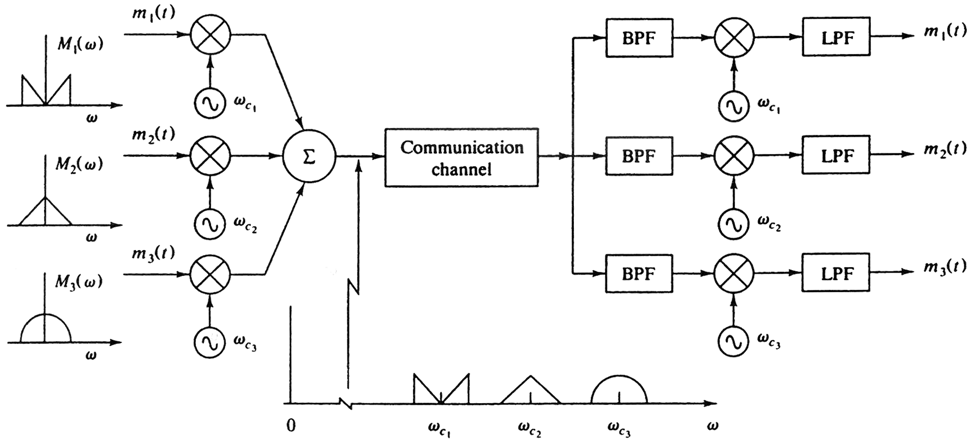
\includegraphics[width=14cm]{bilder/multiplex_fdm_blockdiagramm.png}
\end{center}

\subsection{TDM - Zeitmultiplex (Time-Division Multiplexing)\schaum{100}}
Bei TDM werden mehrere Nachrichtensignale über einen Kommunikationskanal gesendet, indem jedes
einzelne Signal jeweils nur zu bestimmten Zeitintervallen gesendet wird. Diese Umschaltung erfolgt
durch einen sogenannten Commutator. \\
Zeitmultiplex ist das wichtigste Mutiplexingverfahren für
Sprachübertragung inm Telekommunikationsnetz.
\begin{center}
    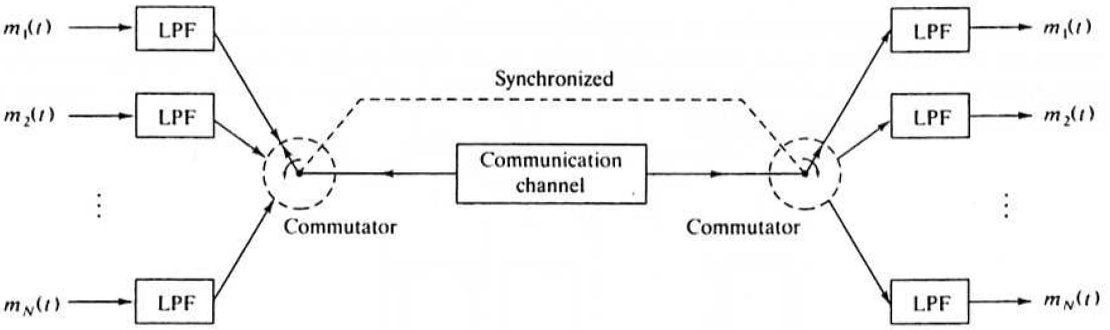
\includegraphics[width=14cm]{bilder/multiplex_tdm_blockdiagramm.png} \\
    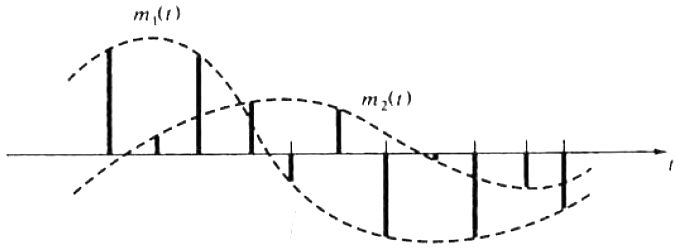
\includegraphics[height=3cm]{bilder/multiplex_tdm_zeitdiagramm.png}     
\end{center}